\documentclass{beamer}
\usepackage{amsmath}
\usepackage[english]{babel} %set language; note: after changing this, you need to delete all auxiliary files to recompile
\usepackage[utf8]{inputenc} %define file encoding; latin1 is the other often used option
\usepackage{csquotes} % provides context sensitive quotation facilities
\usepackage{graphicx} %allows for inserting figures
\usepackage{booktabs} % for table formatting without vertical lines
\usepackage{textcomp} % allow for example using the Euro sign with \texteuro
\usepackage{stackengine}
\usepackage{wasysym}
\usepackage{tikzsymbols}
\usepackage{textcomp}
\newcommand{\bubblethis}[2]{
        \tikz[remember picture,baseline]{\node[anchor=base,inner sep=0,outer sep=0]%
        (#1) {\underline{#1}};\node[overlay,cloud callout,callout relative pointer={(0.2cm,-0.7cm)},%
        aspect=2.5,fill=yellow!90] at ($(#1.north)+(-0.5cm,1.6cm)$) {#2};}%
    }%
\tikzset{face/.style={shape=circle,minimum size=4ex,shading=radial,outer sep=0pt,
        inner color=white!50!yellow,outer color= yellow!70!orange}}
%% Some commands to make the code easier
\newcommand{\emoticon}[1][]{%
  \node[face,#1] (emoticon) {};
  %% The eyes are fixed.
  \draw[fill=white] (-1ex,0ex) ..controls (-0.5ex,0.2ex)and(0.5ex,0.2ex)..
        (1ex,0.0ex) ..controls ( 1.5ex,1.5ex)and( 0.2ex,1.7ex)..
        (0ex,0.4ex) ..controls (-0.2ex,1.7ex)and(-1.5ex,1.5ex)..
        (-1ex,0ex)--cycle;}
\newcommand{\pupils}{
  %% standard pupils
  \fill[shift={(0.5ex,0.5ex)},rotate=80] 
       (0,0) ellipse (0.3ex and 0.15ex);
  \fill[shift={(-0.5ex,0.5ex)},rotate=100] 
       (0,0) ellipse (0.3ex and 0.15ex);}

\newcommand{\emoticonname}[1]{
  \node[below=1ex of emoticon,font=\footnotesize,
        minimum width=4cm]{#1};}
\usepackage{scalerel}
\usetikzlibrary{positioning}
\usepackage{xcolor,amssymb}
\newcommand\dangersignb[1][2ex]{%
  \scaleto{\stackengine{0.3pt}{\scalebox{1.1}[.9]{%
  \color{red}$\blacktriangle$}}{\tiny\bfseries !}{O}{c}{F}{F}{L}}{#1}%
}
\newcommand\dangersignw[1][2ex]{%
  \scaleto{\stackengine{0.3pt}{\scalebox{1.1}[.9]{%
  \color{red}$\blacktriangle$}}{\color{white}\tiny\bfseries !}{O}{c}{F}{F}{L}}{#1}%
}
\usepackage{fontawesome} % Social Icons
\usepackage{epstopdf} % allow embedding eps-figures
\usepackage{tikz} % allows drawing figures
\usepackage{amsmath,amssymb,amsthm} %advanced math facilities
\usepackage{lmodern} %uses font that support italic and bold at the same time
\usepackage{hyperref}
\usepackage{tikz}
\hypersetup{
    colorlinks=true,
    linkcolor=blue,
    filecolor=magenta,      
    urlcolor=blue,
}
\usepackage{tcolorbox}
%add citation management using BibLaTeX
\usepackage[citestyle=authoryear-comp, %define style for citations
    bibstyle=authoryear-comp, %define style for bibliography
    maxbibnames=10, %maximum number of authors displayed in bibliography
    minbibnames=1, %minimum number of authors displayed in bibliography
    maxcitenames=3, %maximum number of authors displayed in citations before using et al.
    minnames=1, %maximum number of authors displayed in citations before using et al.
    datezeros=false, % do not print dates with leading zeros
    date=long, %use long formats for dates
    isbn=false,% show no ISBNs in bibliography (applies only if not a mandatory field)
    url=false,% show no urls in bibliography (applies only if not a mandatory field)
    doi=false, % show no dois in bibliography (applies only if not a mandatory field)
    eprint=false, %show no eprint-field in bibliography (applies only if not a mandatory field)
    backend=biber %use biber as the backend; backend=bibtex is less powerful, but easier to install
    ]{biblatex}
\addbibresource{../mybibfile.bib} %define bib-file located one folder higher


\usefonttheme[onlymath]{serif} %set math font to serif ones

\definecolor{beamerblue}{rgb}{0.2,0.2,0.7} %define beamerblue color for later use

%%% defines highlight command to set text blue
\newcommand{\highlight}[1]{{\color{blue}{#1}}}


%%%%%%% commands defining backup slides so that frame numbering is correct

\newcommand{\backupbegin}{
   \newcounter{framenumberappendix}
   \setcounter{framenumberappendix}{\value{framenumber}}
}
\newcommand{\backupend}{
   \addtocounter{framenumberappendix}{-\value{framenumber}}
   \addtocounter{framenumber}{\value{framenumberappendix}}
}

%%%% end of defining backup slides

%Specify figure caption, see also http://tex.stackexchange.com/questions/155738/caption-package-not-working-with-beamer
\setbeamertemplate{caption}{\insertcaption} %redefines caption to remove label "Figure".
%\setbeamerfont{caption}{size=\scriptsize,shape=\itshape,series=\bfseries} %sets figure  caption bold and italic and makes it smaller


\usetheme{Boadilla}

%set options of hyperref package
\hypersetup{
    bookmarksnumbered=true, %put section numbers in bookmarks
    naturalnames=true, %use LATEX-computed names for links
    citebordercolor={1 1 1}, %color of border around cites, here: white, i.e. invisible
    linkbordercolor={1 1 1}, %color of border around links, here: white, i.e. invisible
    colorlinks=true, %color links
    anchorcolor=black, %set color of anchors
    linkcolor=beamerblue, %set link color to beamer blue
    citecolor=blue, %set cite color to beamer blue
    pdfpagemode=UseThumbs, %set default mode of PDF display
    breaklinks=true, %break long links
    pdfstartpage=1 %start at first page
    }


% --------------------
% Overall information
% --------------------
\title[Principios de Economía]{Principios de Economía}
\date{}
\author[Ertola y Sturzenegger]{Gabriela Ertola y Federico Sturzenegger }
\vspace{0.4cm}
\institute[]{Universidad de San Andrés \\
2022} 

\begin{document}

\begin{frame}
\titlepage
\centering

\includegraphics[scale=0.25]{Figures/logoUDESA.jpg} 
\end{frame}

\begin{frame}
\frametitle{Estructura del programa}
\begin{itemize}
\begin{itemize}
    \item Introducción
    \item Escasez y elección
    \itemInteracciones sociales
    \item Instituciones, poder, ganadores y perdedores
    \item Dentro de la firma
    \item Firmas eligiendo precio y cantidad
    \item Tomando precios
    \item Mercado laboral
    \item Crédito, dinero y bancos
    \item Fallas de mercado
    \item Fluctuaciones económicas
    \item Política fiscal
    \item Política monetaria
\end{itemize}
\end{itemize}
\end{frame}

\begin{frame}
\frametitle{1. Juego de libre asociación}
\begin{itemize}
    \item Ingresen a www.menti.com
    \item Usen el código 3765 0331 
    \item Ingresen 3 palabras que asocien con economía
\end{itemize} 
    \begin{center}
    
\includegraphics[scale=0.3]{Figures/menti.png}
    \end{center}
\end{frame}

\begin{frame}
\frametitle{2. ¿Qu\'{e} es la economía?}
\begin{itemize}
    \item Etimología de la palabra economía 
    \item Es una ciencia: tiene un objeto propio (fenómenos económicos), un método (inductivo - deductivo) y un conjunto de teorías económicas capaces de explicar estos fenómenos
    \item Es una ciencia empírica: se puede contrastar con la realidad 
    \item Es una ciencia social: estudia diversos aspectos de las sociedades
    \vspace{2mm}
\end{itemize}
\end{frame}

\begin{frame}
\frametitle{3. ¿Qu\'{e} es la economía?}
ESTO NO...\vspace{1mm} \\
\centering 
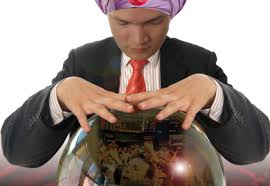
\includegraphics[scale=0.7]{Figures/Introduccion_1.2_boladecristal.jpg}
\\
¡No es una ciencia exacta!
\end{frame}

\begin{frame}
\frametitle{4. ¿Qu\'{e} hace un economista?}
\begin{itemize}
    \item Busca asignar eficientemente recursos escasos \vspace{3mm} \\
    \item ¿Que quiere decir `eficientemente'? \vspace{3mm} \\
    \item ¿Qué mecanismos tiene para realizar dicha asignación? 
\end{itemize}
\end{frame}

\begin{frame}
\frametitle{5. ¿Qu\'{e} aspectos estudia la economía?}
\begin{itemize}
\begin{itemize}
    \item Cómo llegamos a adquirir las cosas \vspace{2mm}
    \item Cómo interactuamos unos con otros (compradores y vendedores, empleados y empleadores, ciudadanos y servidores públicos, padres, hijos y familia) \vspace{2mm}
    \item Cómo interactuamos con nuestro medioambiente \vspace{2mm}
    \item Cómo estas cosas cambian en el tiempo  
\end{itemize}
\end{itemize}
\end{frame}

\begin{frame}
\frametitle{6. Entendiendo el mundo}
Estudiar las causas y consecuencias de los problemas sociales es un reto 
\begin{itemize}
    \item Responder algunas preguntas no es fácil...
    \begin{itemize}
        \item ¿Por qué algunos países son ricos y otros son pobres?
        \item ¿Por qué hay inflación en Argentina?
        \item ¿Las mujeres que se casan más tarde tienen niños más educados?
        \item ¿Causan los cinturones de seguridad más accidentes?
        \end{itemize}
    \item ¡A veces es complicado comprender la pregunta!
\end{itemize}
\end{frame}

\begin{frame}
\frametitle{7. ¿Cómo hacer frente a estas preguntas?}
    \begin{itemize}
            \item Vamos a pensar utilizando modelos económicos... \vspace{2mm}
            \item y vamos confrontar esos modelos con la realidad
    \end{itemize} \vspace{2mm}
En este proceso, vamos a usar herramientas cuantitativas y representaciones gráficas \vspace{2mm}
    \begin{itemize}
        \item Para describir la realidad y mostrar relaciones entre variables reales
        \item Ser transparente con la teorías que se elaboran
        \end{itemize}
\end{frame}

\begin{frame}
\frametitle{8. ¿Qué es un modelo?}
\begin{itemize}
    \item El mundo es muy complejo! Para entenderlo debemos simplificar la realidad \vspace{2mm} \\ $\Rightarrow$
    Supuestos y modelos \vspace{2mm}
    \item ¿Que es un modelo? Es una simplificación de la realidad \vspace{2mm}
    \item  \href{https://www.youtube.com/watch?v=zwDA3GmcwJU}{``Del rigor de la ciencia''} 
    Jorge Luis Borges
\end{itemize}
\end{frame}

\begin{frame}
\frametitle{9. ¿Cómo construimos modelos?}
\begin{itemize}
    \item Construimos una descripción simplificada de las condiciones bajo las cuales la gente lleva a cabo sus acciones \vspace{2mm}
    \item Describimos en términos simples qué determina las acciones que la gente toma \vspace{2mm}
    \item Determinamos cómo sus acciones afectan a otros
\end{itemize} 
\end{frame}

\begin{frame}
\frametitle{10. ¿Cómo construimos modelos?}
\begin{itemize}
    \item Determinamos el resultado de estas acciones, cosa que resulta a veces en un equilibrio (algo constante) \vspace{2mm}
    \item Finalmente, tratamos de obtener mayor profundidad al estudiar qué ocurre cuando las condiciones cambian 
\end{itemize} 
\end{frame}

\begin{frame}
\frametitle{11. ¿Qué es un buen modelo?}
\begin{itemize}
    \item Es claro: nos ayuda a entender algo importante
    \item Predice con precisión: sus predicciones son consistentes con la evidencia \vspace{1mm}
    \item Mejora la comunicación. Nos ayuda a entender en qué estamos de acuerdo (y qué en desacuerdo) \vspace{1mm}
    \item Es útil. Podemos usarlo para encontrar formas de mejorar el funcionamiento de la economía
\end{itemize} 
\end{frame}

\begin{frame}
\frametitle{12. ¿Por qué vamos a usar gráficos?}
\begin{itemize}
    \item Los gráficos sirven para mostrar ideas \vspace{2mm}
    \item Los gráficos son útiles para ver si hay relación entre dos variables 
     \begin{itemize}
        \item ¡Pero tenemos que tener cuidado! Esas relaciones dan indicios de correlación... pero no de causalidad! \vspace{2mm}
    \end{itemize}
    \item Los gráficos (y sus expresiones matemáticas) pueden ser utilizados para describir una teoría
\end{itemize} 
\end{frame}

\begin{frame}
\frametitle{13. La correlación...}
\begin{center}
    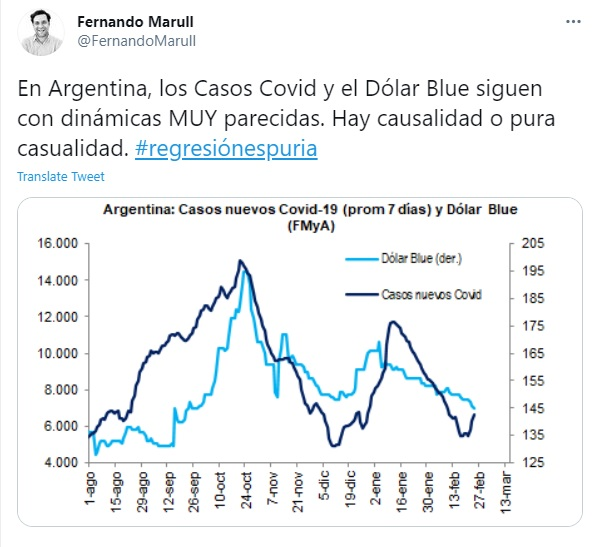
\includegraphics[scale=0.55]{Figures/Introduccion_1.3.jpg}
\end{center}
\end{frame}

\begin{frame} \label{uno}
\frametitle{14. Algunas explicaciones}
\begin{itemize}
    \item OJO al interpretar relaciones entre variables porque \hyperlink{hdos}{correlación no implica causalidad}   \vspace{2mm}
    \item Endogeneidad: ``todo tiene que ver con todo'' \vspace{1mm}
    \begin{itemize} 
        \item Potenciales fuentes de sesgo:
        \begin{itemize}
            \item \hyperlink{htres}{Omisión de variables}  
            \item \hyperlink{hcuatro}{Simultaneidad} 
            \item \hyperlink{hcinco}{Error de medición en la variable explicativa}
        \end{itemize}
    \end{itemize}
\end{itemize}
\end{frame}

\begin{frame} 
\frametitle{15.¿Qué podemos hacer?}
\begin{itemize}
    \item  En algunos casos se pueden diseñar experimentos o utilizar experimentos naturales (exógenos por definición) para detectar eventos que producen un cambio claro en la variable independiente
\end{itemize}
\end{frame}

\begin{frame} 
\frametitle{16. Un ejemplo más}
\begin{center}
    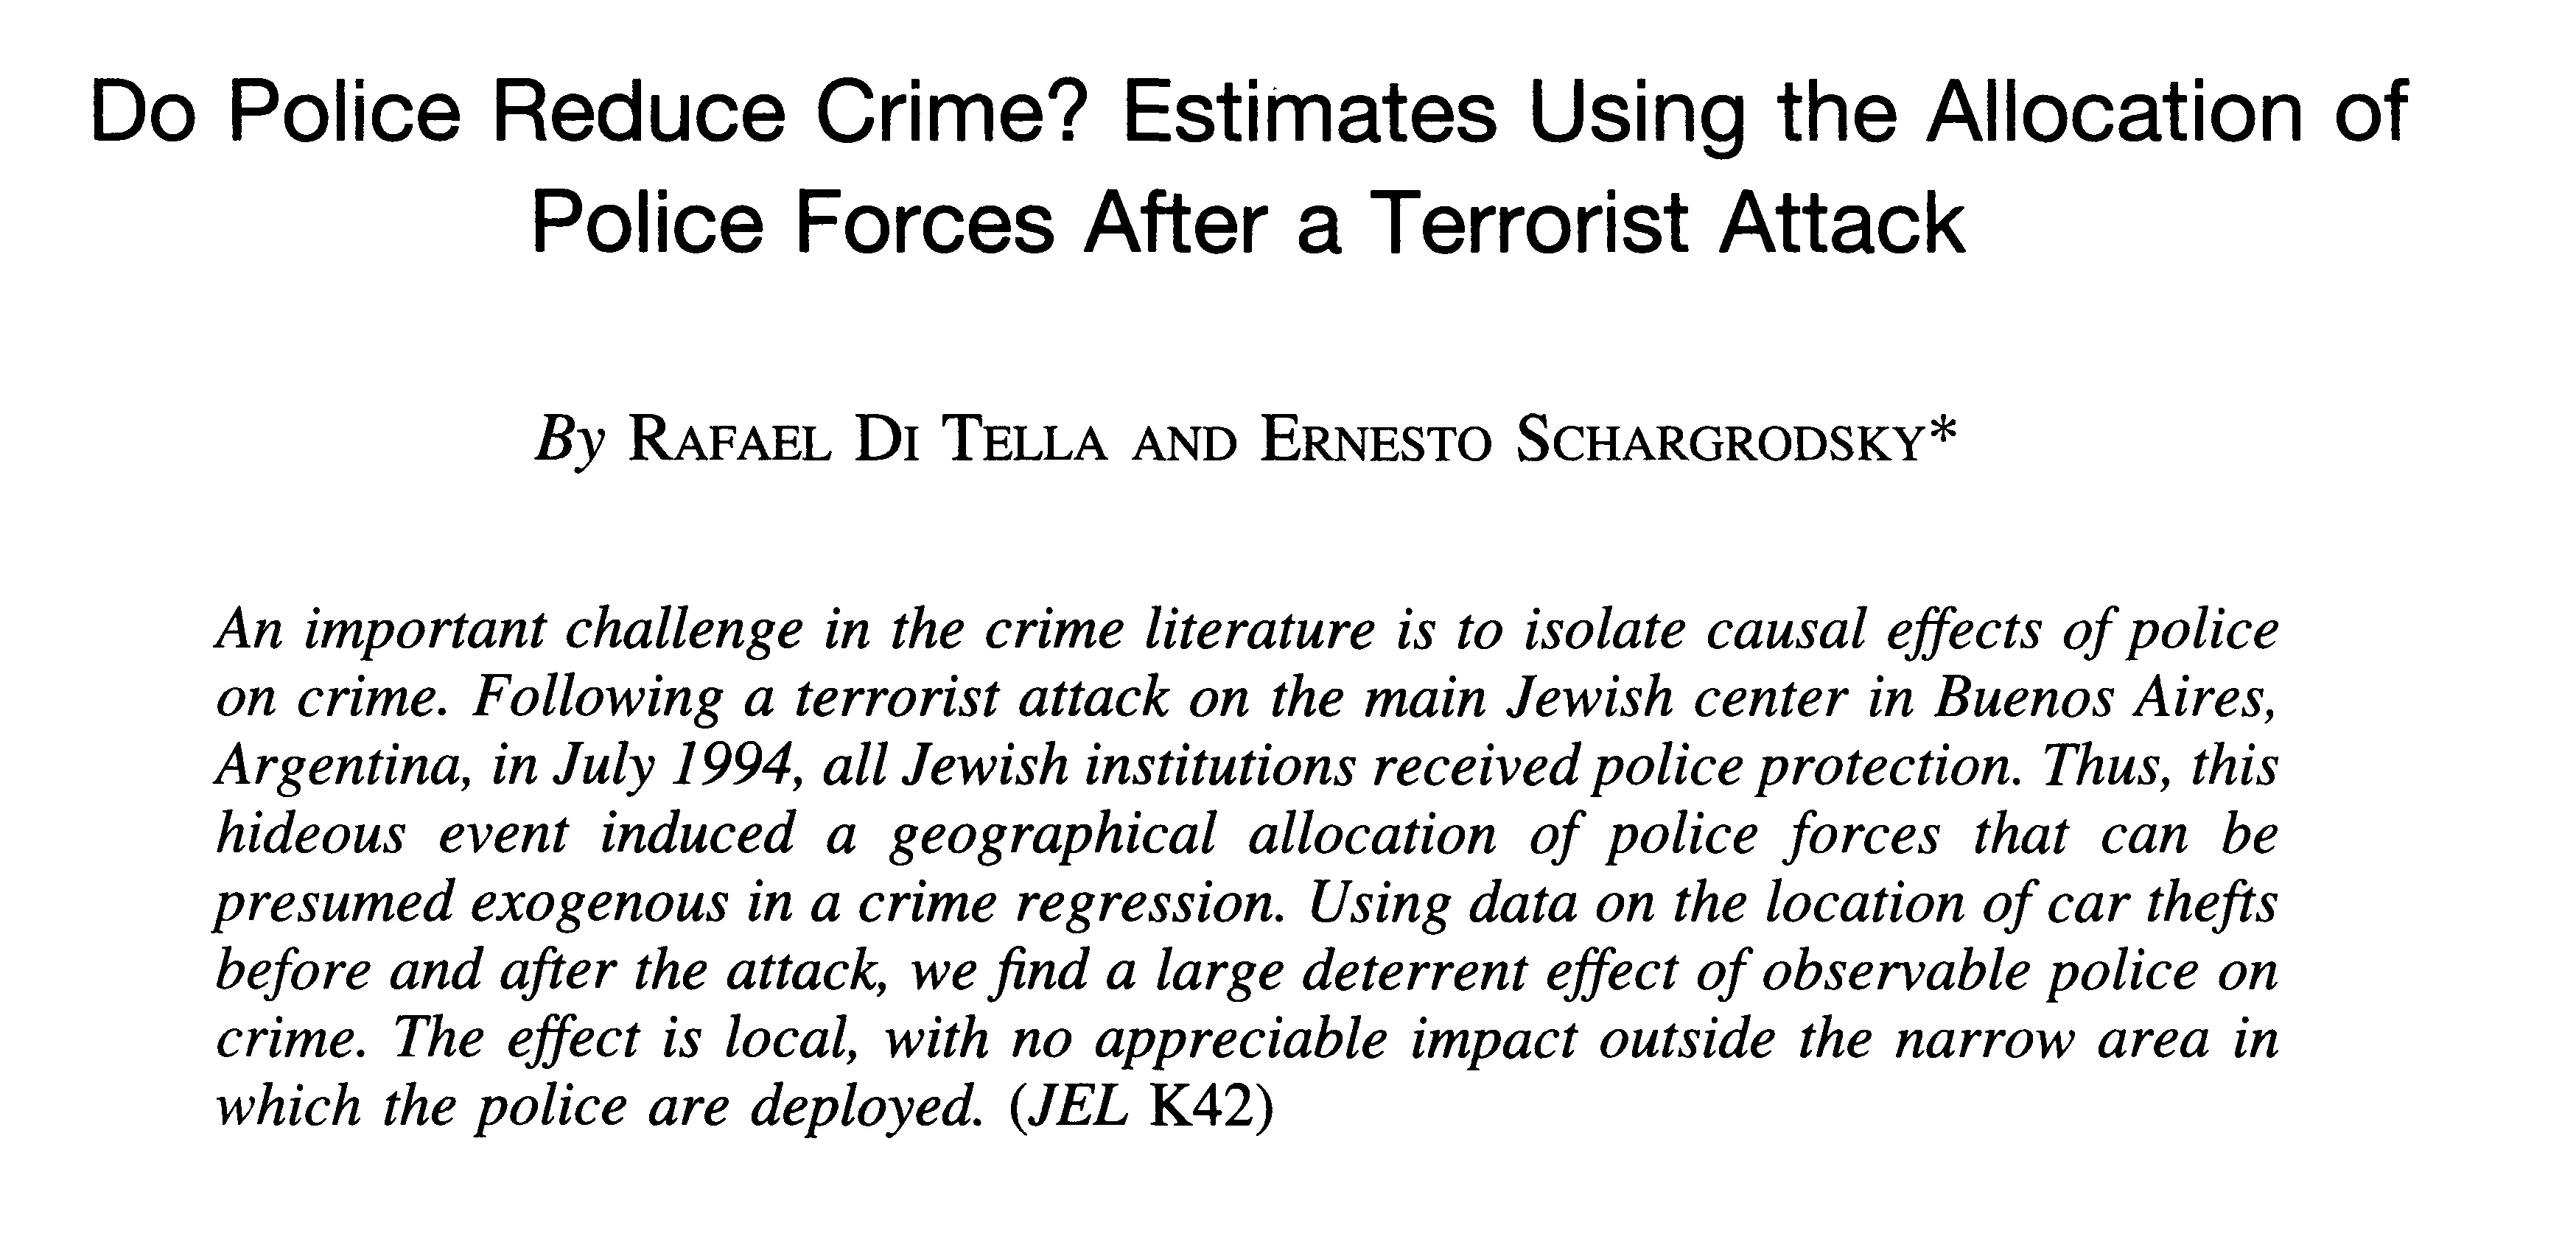
\includegraphics[scale=0.12]{Figures/Introduccion_1.7_Dopolice.jpg}
\end{center}
\end{frame}

%%%%%%%%%%%%%%%%%%%%%%%%%%%%%%%%%%%%%%%%%%%%%%%%%%%%%%%%%%
%\begin{frame}
%\frametitle{14. Si están interesados y con un poquito de tiempo libre pueden explorar...}
%\large
%\href{http://www.gapminder.org}{GAPMINDER} %\url{https://www.gapminder.org} 
%\end{frame}

\begin{frame} \label{hdos}
\frametitle{Correlación versus Causalidad}
\begin{center}
    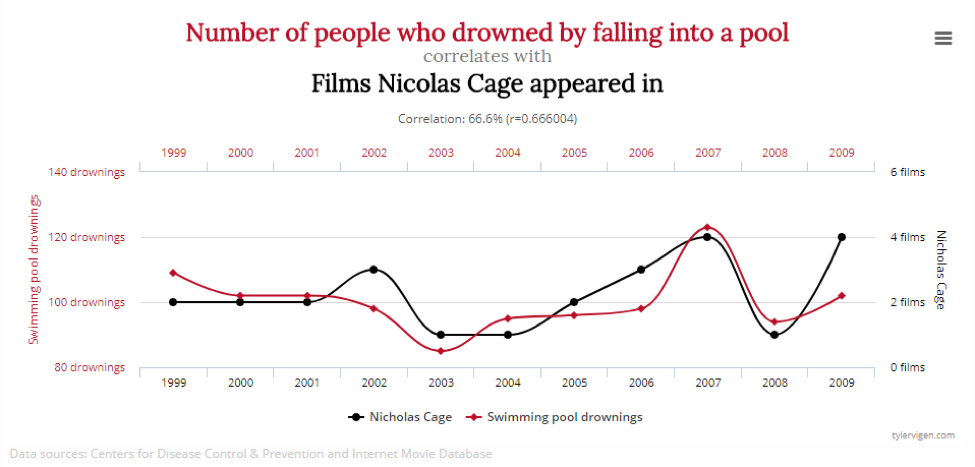
\includegraphics[scale=0.3]{Figures/Introduccion_1.4.1_corrcaus.png}
\end{center}
Fuente: Google \\
\hyperlink{uno}{Volver} 
\end{frame}

\begin{frame} \label{htres}
\frametitle{Correlación versus Causalidad}
\begin{center}
    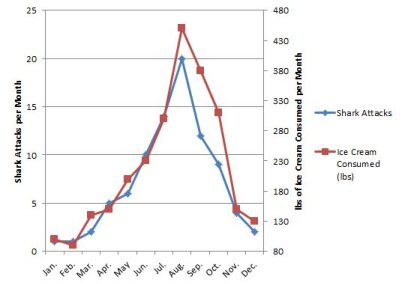
\includegraphics[scale=0.55]{Figures/Introduccion_1.5_ovbias.jpg}
\end{center}
Fuente: Google \\
\hyperlink{uno}{Volver} 
\end{frame}

\begin{frame} \label{hcuatro}
\frametitle{Correlación versus Causalidad}
\begin{center}
    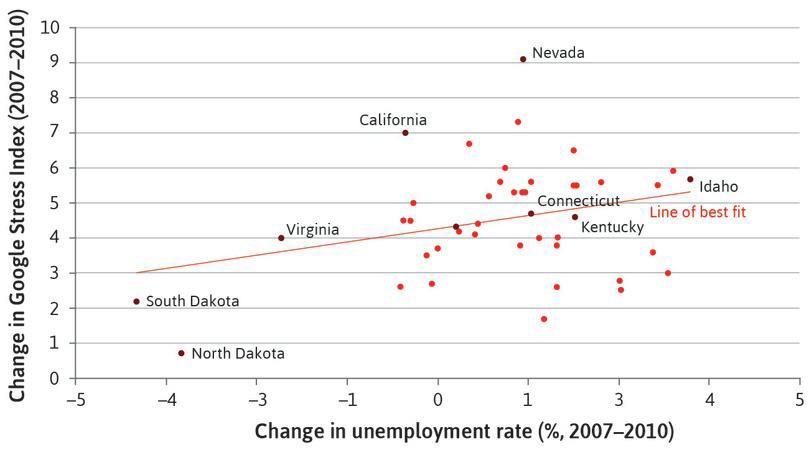
\includegraphics[scale=0.35]{Figures/Introduccion_1.3_desempleoestres.jpg}
\end{center}
Fuente: Google \\
\hyperlink{uno}{Volver} 
\end{frame}

\begin{frame} \label{hcinco}
\frametitle{Correlación versus Causalidad}
\begin{center}
    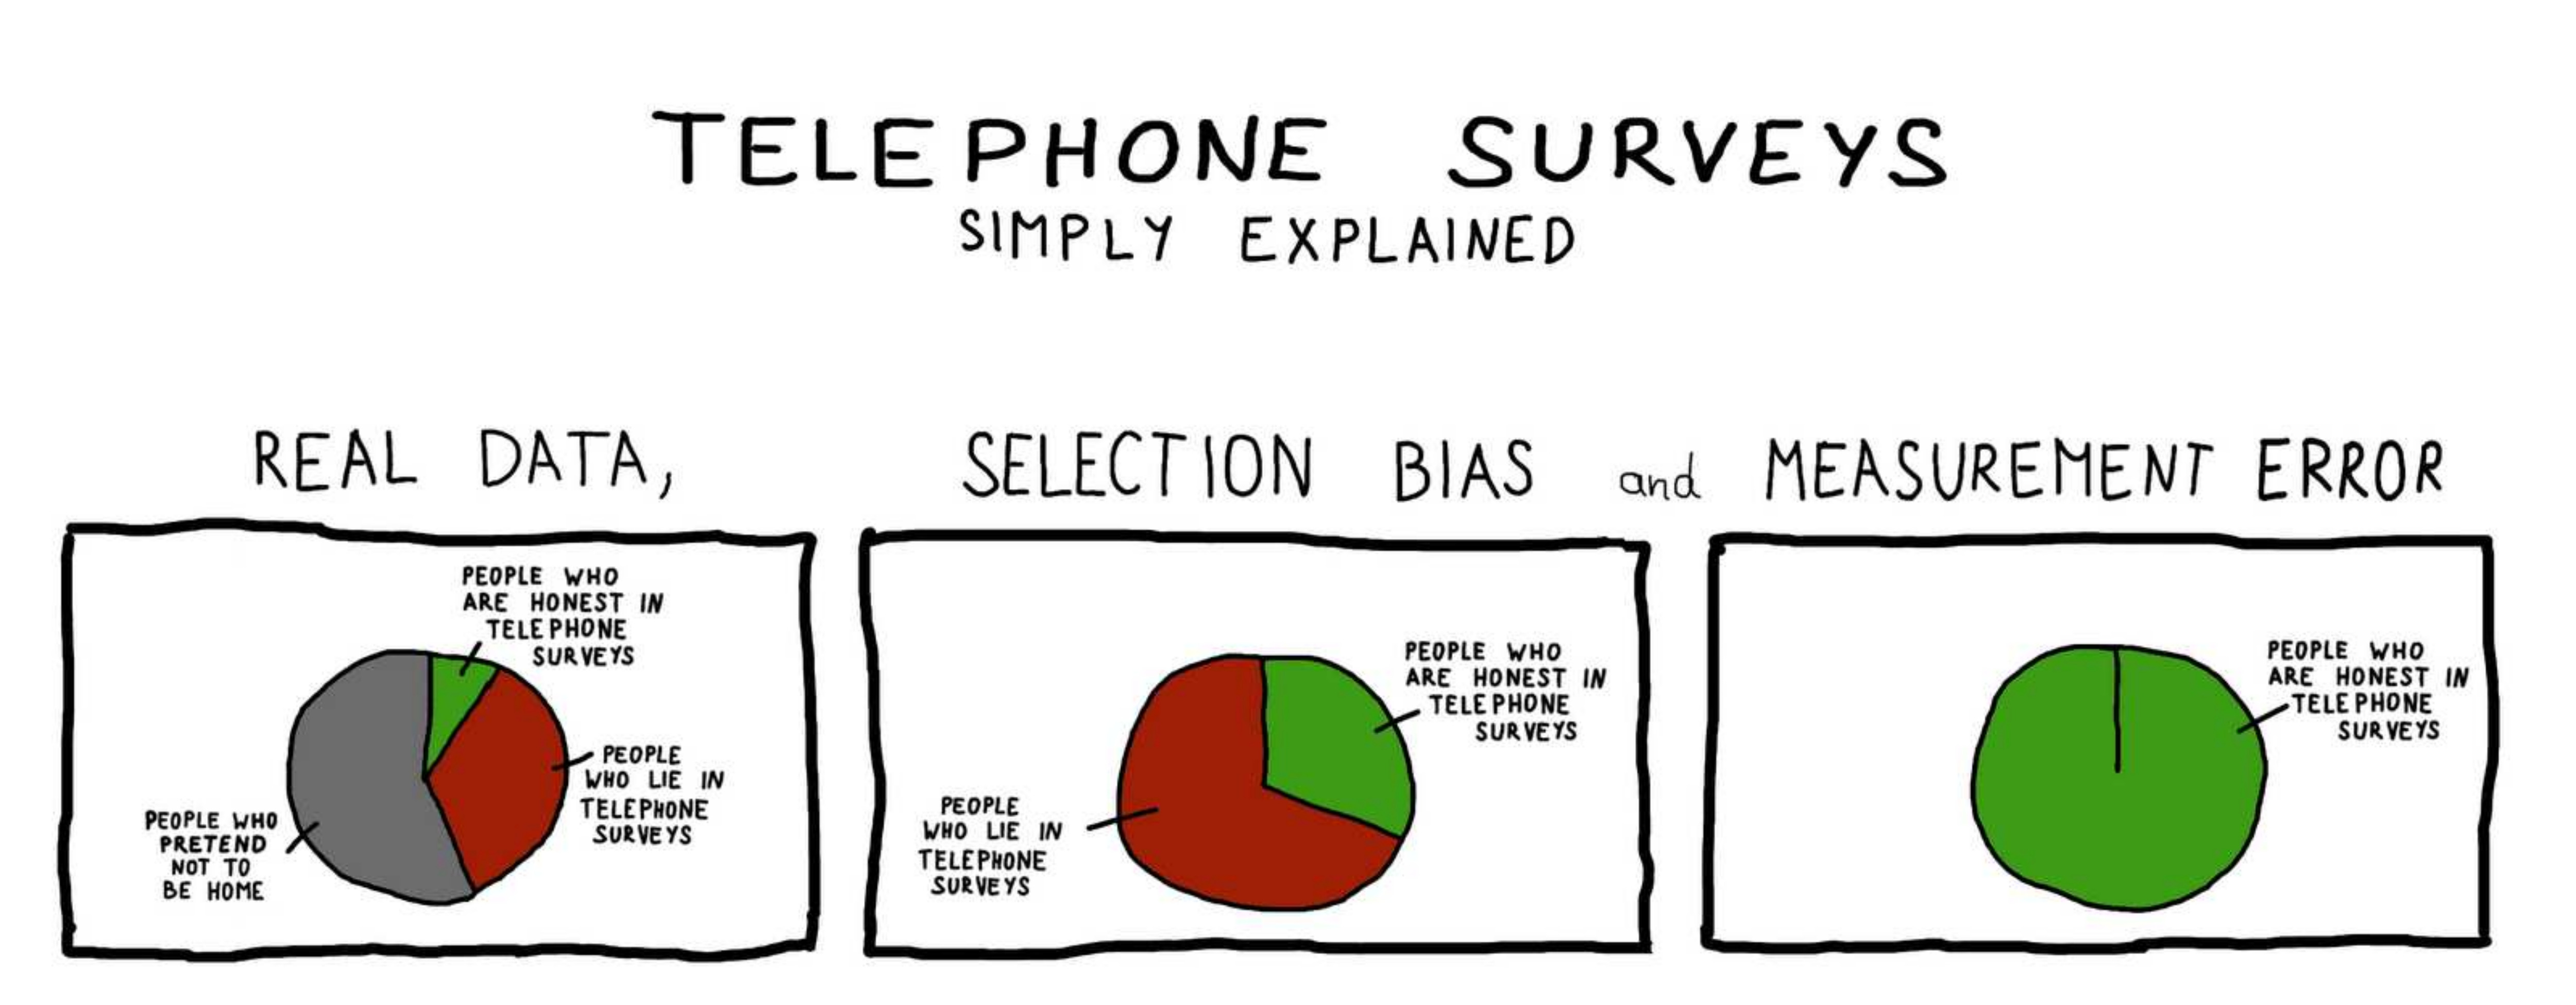
\includegraphics[scale=0.25]{Figures/Introduccion_1.6_errormedicion.jpg}
\end{center}
Fuente: Google \\
\hyperlink{uno}{Volver} 
\end{frame}




\end{document}




